%
%===============>>  ГРУППА 9-2 МОДУЛЬ 6  <<=============
%
\setmodule{6}

%BEGIN_FOLD % ====>>_____ Занятие 1 _____<<====
\begin{class}[number=1]
	\begin{listofex}
		\item В таблице даны размеры (с точностью до мм) четырёх листов, имеющих форматы \( A0 \), \( A1 \), \( A3 \), \( A4 \).
		\begin{center}
			\footnotesize
			\begin{tabular}{|c|c|c|}
				\hline
				\rowcolor{gray}\textbf{Номер листа}&\textbf{Длина(мм)}&\textbf{Ширина мм}\\
				\hline
				\( 1 \)&\( 297 \)&\( 210 \)\\
				\hline
				\( 2 \)&\( 420 \)&\( 297 \)\\
				\hline
				\( 3 \)&\( 1189 \)&\( 841 \)\\
				\hline
				\( 4 \)&\( 841 \)&\( 594 \)\\
				\hline
			\end{tabular}
		\end{center}
		Установите соответствие между форматами и номерами листов. В ответ запишите последовательность четырёх цифр, соответствующих номерам листов, без пробелов, запятых и дополнительных символов.
		\begin{center}
			\footnotesize
			\begin{tabular}{|c|c|c|c|}
				\hline
				\textbf{\( A0 \)}&\textbf{\( A1 \)}&\textbf{\( A3 \)}&\textbf{\( A4 \)}\\
				\hline
				\(  \)&\(  \)&\(  \)&\(  \)\\
				\hline
			\end{tabular}
		\end{center}
		Общепринятые форматы листов бумаги обозначают буквой \( A \) и цифрой: \( A0 \), \( A1 \), \( A2 \) и так далее. Лист формата \( A0 \) имеет форму прямоугольника, площадь которого равна \( 1 \) кв. м. Если лист формата А0 разрезать пополам параллельно меньшей стороне, получается два равных листа формата \( A1 \). Если лист \( A1 \) разрезать так же пополам, получается два листа формата \( A2 \). И так далее.\\
		\begin{minipage}[c]{0.35\textwidth}
			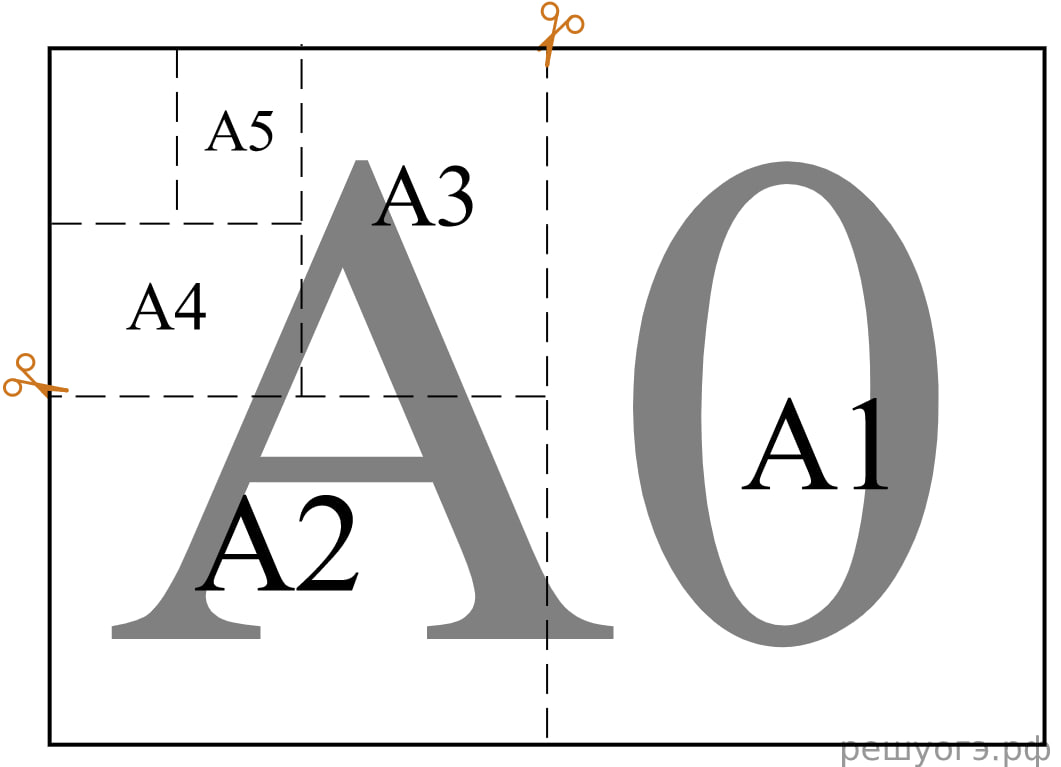
\includegraphics[align=t, width=\linewidth]{\picpath/G91M6L1}
		\end{minipage}\\
		Отношение большей стороны к меньшей стороне листа каждого формата одно и то же, поэтому листы всех форматов подобны. Это сделано специально для того, чтобы пропорции текста и его расположение на листе сохранялись при уменьшении или увеличении шрифта при изменении формата листа.
		\item Сколько листов формата \( A3 \) получится из одного листа формата \( A2 \)?
		\item Найдите площадь листа формата \( A1 \). Ответ дайте в квадратных сантиметрах.
		\item Найдите отношение длины меньшей стороны листа формата \( A3 \) к большей. Ответ округлите до десятых.
		\item Бумагу формата \( A5 \) упаковали в пачки по \( 500 \) листов. Найдите массу пачки, если масса бумаги площади \( 1 \) кв. м равна \( 80 \) г. Ответ дайте в граммах.
		\item Диагональ \( BD \) параллелограмма \( ABCD \) образует с его сторонами углы, равные \( 65\degree \) и \( 50\degree \). Найдите меньший угол параллелограмма.
		\item На продолжении стороны \( AD \) параллелограмма \( ABCD \) за точкой \( D \) отмечена точка \( E \) так, что \( DC=DE \). Найдите больший угол параллелограмма \( ABCD \), если \( \angle DEC=53\degree \). Ответ дайте в градусах.
		\item В параллелограмм вписана окружность. Найдите периметр параллелограмма, если одна из его сторон равна \( 6 \).
		\item Биссектриса угла \( A \) параллелограмма \( ABCD \) пересекает сторону \( BC \) в точке \( K \). Найдите периметр параллелограмма, если \( BK=6 \), \( CK=10 \).
		\item Площадь параллелограмма равна \( 40 \), а две его стороны равны \( 5 \) и \( 10 \). Найдите его высоты. В ответе укажите большую высоту.
		\item Расстояние от точки пересечения диагоналей ромба до одной из его сторон равно \( 19 \), а одна из диагоналей ромба равна \( 76 \). Найдите углы ромба.
		\item Периметр прямоугольника равен 56, а диагональ равна 27. Найдите площадь этого прямоугольника.
		\item Одна из сторон параллелограмма равна \( 12 \), другая равна \( 5 \), а косинус одного из углов равен \( \dfrac{2\sqrt{2}}{3} \). Найдите площадь параллелограмма.
		\item В ромбе сторона равна \( 10 \), одна из диагоналей --- \( 10\sqrt{2+\sqrt{2}} \), а угол, лежащий напротив этой диагонали, равен \( 135\degree \). Найдите площадь ромба, деленную на \( \sqrt{2} \).
		\item Площадь параллелограмма \( ABCD \) равна \( 132 \). Точка \( E \) --- середина стороны \( AB \). Найдите площадь треугольника \( CBE \).
		\item Площадь ромба равна \( 54 \), а периметр равен \( 36 \). Найдите высоту ромба.
	\end{listofex}
\end{class}
%END_FOLD

%BEGIN_FOLD % ====>>_____ Занятие 2 _____<<====
\begin{class}[number=2]
	\begin{listofex}
		\item Установите соответствие между объёмами помещения и номерами печей, для которых данный объём является наименьшим для отопления помещений. Заполните таблицу, в бланк ответов перенесите последовательность трёх цифр без пробелов, запятых и других дополнительных символов.
		\begin{center}
			\footnotesize
			\begin{tabular}{|c|c|c|c|}
				\hline
				Объём&\( 8 \)&\( 9 \)&\( 10 \)\\
				\hline
				Номер печи&\(  \)&\(  \)&\(  \)\\
				\hline
			\end{tabular}
		\end{center}
		Хозяин дачного участка строит баню с парным отделением. Парное отделение имеет размеры: длина \( 3,5 \) м, ширина \( 2,2 \) м, высота \( 2 \) м. Окон в парном отделении нет, для доступа внутрь планируется дверь шириной \( 60 \) см, высота дверного проёма \( 1,8 \) м. Для прогрева парного отделения можно использовать электрическую или дровяную печь. В таблице представлены характеристики трёх печей.
		\begin{center}
			\footnotesize
			\begin{tabular}{|c|c|c|c|c|}
				\hline
				\rowcolor{gray}\textbf{Номера печи}&\textbf{Тип}&\textbf{Объём помещения}&\textbf{Масса}&\textbf{Стоимость}\\
				\hline
				1&Дровяная&\( 8-12 \)&\( 40 \)&\( 18 000 \)\\
				\hline
				2&Дровяная&\( 10-16 \)&\( 48 \)&\( 19 500 \)\\
				\hline
				3&Электрическая&\( 9-15,5 \)&\( 15 \)&\( 15 000 \)\\
				\hline
			\end{tabular}
		\end{center}
		Для установки дровяной печи дополнительных затрат не потребуется. Установка электрической печи потребует подведения специального кабеля, что обойдётся в \( 6500 \) руб.
		\item Найдите объём парного отделения строящейся бани. Ответ дайте в кубических метрах.
		\item На сколько рублей покупка дровяной печи, подходящей по объёму парного отделения, обойдётся дороже электрической без учёта установки?
		\item Во сколько рублей обойдётся покупка электрической печи с установкой и доставкой, если доставка печи до дачного участка будет стоить \( 800 \) рублей?
		\item На дровяную печь, масса которой \( 48 \) кг, сделали скидку \( 10\% \). Сколько рублей стала стоить печь?
		\item Хозяин выбрал дровяную печь (рис. \( 1 \)). Чертёж передней панели печи показан на рисунке \( 2 \).
		\begin{minipage}[c]{0.35\textwidth}
			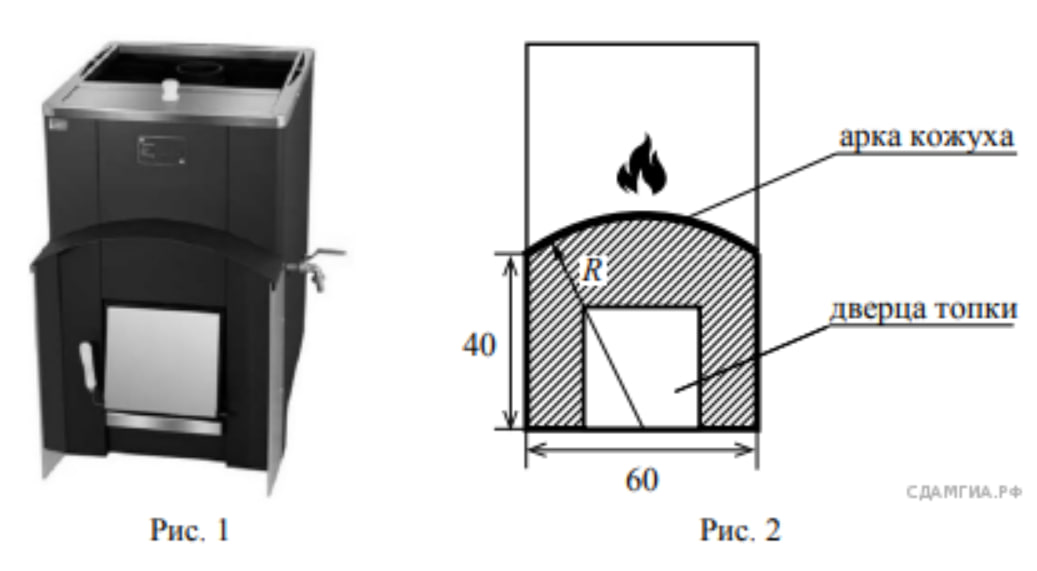
\includegraphics[align=t, width=\linewidth]{\picpath/G91M6L2}
		\end{minipage}\\
		Печь снабжена кожухом вокруг дверцы топки. Верхняя часть кожуха выполнена в виде арки, приваренной к передней стенке печки по дуге окружности с центром в середине нижней части кожуха (см. рис. \( 2 \)). Для установки печки хозяину понадобилось узнать радиус закругления арки \( R \). Размеры кожуха в сантиметрах показаны на рисунке. Найдите радиус закругления арки в сантиметрах.
		\item Расстояние между пристанями \( A \) и \( B \) равно \( 80 \) км. Из \( A \) в \( B \) по течению реки отправился плот, а через \( 2 \) часа вслед за ним отправилась яхта, которая, прибыв в пункт \( B \), тотчас повернула обратно и возвратилась в \( A \). К этому времени плот прошел \( 22 \) км. Найдите скорость яхты в неподвижной воде, если скорость течения реки равна \( 2 \) км/ч. Ответ дайте в км/ч.
		\item Расстояние между городами \( A \) и \( B \) равно \( 750  \) км. Из города \( A \) в город \( B \) со скоростью \( 50 \) км/ч выехал первый автомобиль, а через три часа после этого навстречу ему из города \( B \) выехал со скоростью \( 70 \) км/ч второй автомобиль. На каком расстоянии от города \( A \) автомобили встретятся?	
		\item 
		\begin{minipage}[t]{\bodywidth}
			В параллелограмме \( ABCD \) проведены перпендикуляры \( DE \) и \( DF \) к диагонали \( AC \) (см. рис.). Докажите, что \( BFDE \) --- параллелограмм.
		\end{minipage}
		\hspace{0.02\linewidth}
		\begin{minipage}[t]{\picwidth}
			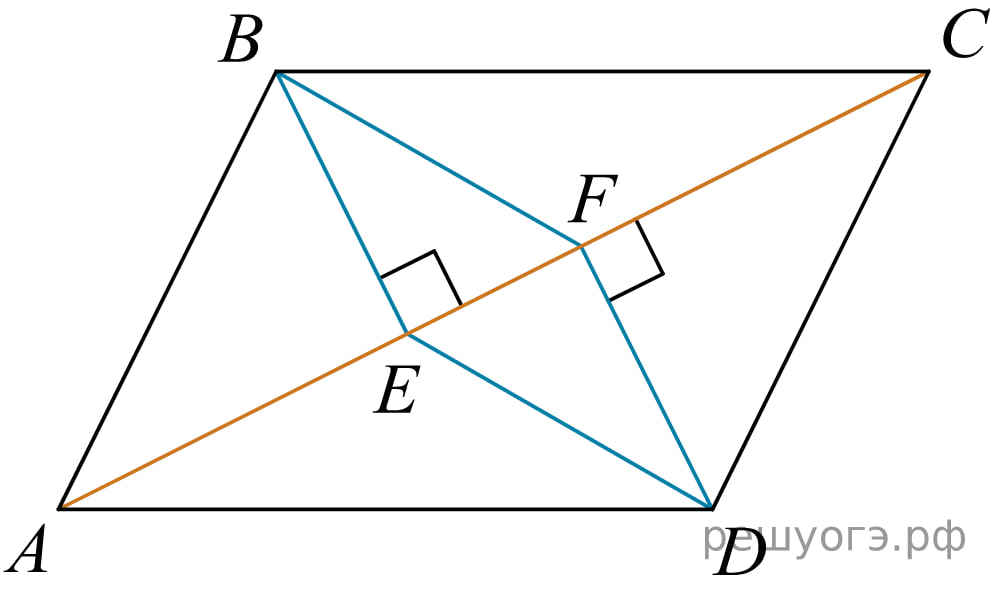
\includegraphics[align=t, width=\linewidth]{\picpath/G92M6L2}
		\end{minipage}
		\item Сторона \( BC \) параллелограмма \( ABCD \) вдвое больше стороны \( CD \). Точка \( L \) --- середина стороны \( BC \). Докажите, что \( DL \) --- биссектриса угла \( CDA \).
	\end{listofex}
\end{class}
%END_FOLD

%BEGIN_FOLD % ====>>_ Домашняя работа 1 _<<====
\begin{homework}[number=1]
	\begin{listofex}
		\item Домашняя работа 1
	\end{listofex}
\end{homework}
%END_FOLD

%BEGIN_FOLD % ====>>_____ Занятие 3 _____<<====
\begin{class}[number=3]
	\begin{listofex}
		\item Занятие 3 
	\end{listofex}
\end{class}
%END_FOLD

%BEGIN_FOLD % ====>>_____ Занятие 4 _____<<====
\begin{class}[number=4]
	\begin{listofex}
		\item Занятие 4
	\end{listofex}
\end{class}
%END_FOLD

%BEGIN_FOLD % ====>>_ Домашняя работа 2 _<<====
\begin{homework}[number=2]
	\begin{listofex}
		\item Домашняя работа 2
	\end{listofex}
\end{homework}
%END_FOLD

%BEGIN_FOLD % ====>>_____ Занятие 5 _____<<====
\begin{class}[number=5]
	\begin{listofex}
		\item Занятие 5
	\end{listofex}
\end{class}
%END_FOLD

%BEGIN_FOLD % ====>>_____ Занятие 6 _____<<====
\begin{class}[number=6]
	\begin{listofex}
		\item Занятие 6
	\end{listofex}
\end{class}
%END_FOLD

%BEGIN_FOLD % ====>>_ Домашняя работа 3 _<<====
\begin{homework}[number=3]
	\begin{listofex}
		\item Домашняя работа 3
	\end{listofex}
\end{homework}
%END_FOLD

%BEGIN_FOLD % ====>>_____ Занятие 7 _____<<====
\begin{class}[number=7]
	\title{Подготовка к проверочной}
	\begin{listofex}
		\item Занятие 7
	\end{listofex}
\end{class}
%END_FOLD

%BEGIN_FOLD % ====>>_ Проверочная работа _<<====
\begin{exam}
	\begin{listofex}
		\item Проверочная
	\end{listofex}
\end{exam}
%END_FOLD